\documentclass{article}

\usepackage[utf8]{inputenc}
\usepackage[brazilian]{babel}
\usepackage{graphicx}
\usepackage{float}
\usepackage[pdftex]{hyperref}
\usepackage{epstopdf}
\usepackage{etoolbox}
\usepackage{amsmath}
\usepackage{amsfonts}
\usepackage{amssymb}
\usepackage{caption}
\usepackage{subcaption}
\usepackage{setspace}
\usepackage{tikz}

\patchcmd{\thebibliography}{\section*}{\section}{}{}
\newcommand{\R}{\ensuremath{\mathbb{R}}}
\newcommand{\Prob}{\ensuremath{\mathbb{P}}}
\newcommand{\K}{\ensuremath{\mathbb{K}}}
\newcommand{\U}{\ensuremath{\mathbb{U}}}
\newcommand{\N}{\ensuremath{\mathbb{N}}}
\newcommand{\Lg}{\ensuremath{\mathbb{L}}}
\newcommand{\T}{\ensuremath{\rm Tr}}
\newcommand{\sg}{{\sigma(x_k)}}

\newcommand{\G}{\ensuremath{\mathcal{G}}}
\newcommand{\F}{\ensuremath{\mathcal{F}}}
\newcommand{\C}{\ensuremath{\mathcal{C}}}
\newcommand{\E}{\ensuremath{\mathcal{E}}}
\newcommand{\Hn}{\ensuremath{\mathcal{H}}}
%\newcommand{\Hoo}{\ensuremath{\mathcal{H}_\infty}}
\newcommand{\Hop}{\ensuremath{\mathcal{H}_{op}}}
% --------------------------------------------------
\newtheorem{theo}{Teorema}
\newtheorem{exa}{Exemplo}
\newtheorem{lemm}{Lema}
\newtheorem{coro}{Corolário}
\newtheorem{defn}{Definição}[section]

%opening


\begin{document}

\begin{titlepage}
\begin{center}

\newcommand{\HRule}{\rule{\linewidth}{0.5mm}}
% Upper part of the page. The '~' is needed because \\
% only works if a paragraph has started.

\includegraphics[width=0.15\textwidth]{logounicamp.pdf}~\\[1cm]

\textsc{\LARGE Universidade Estadual de Campinas}\\[1.5cm]

\textsc{\Large Faculdade de Engenharia Mecânica}\\[0.5cm]

% Title
\HRule \\[0.4cm]
{ \huge \bfseries ES828 - Laboratório de Controle de Sistemas\\ \vspace{1cm} Relatório - Experimento 2 \\
\Large{Método de identificação de plantas eletrônicas} \\[0.4cm] }

\HRule \\[1.5cm]

% Author and supervisor
\begin{minipage}{0.6\textwidth}
\begin{flushleft} \large
\emph{Nome:}\\
Daniel Dello Russo Oliveira\\ Marcelli Tiemi Kian
\end{flushleft}
\end{minipage}
\begin{minipage}{0.2\textwidth}
\begin{flushright} \large
\emph{RA}\\ 101918\\
117892
\end{flushright}
\end{minipage}

\vfill

% Bottom of the page
{\large \today}

\end{center}
\end{titlepage}


\onehalfspacing
\section{Objetivos} 
O objetivo desse experimento é a familiarização com o projeto de controladores PID e o estudo do seu desempenho.
	
\section{Projeto dos Controladores}
Devido a problemas encontrados com os controladores projetados no pré relatório do experimento três \cite{bb:prelab3}, nós refizemos as medidas do experimento dois e determinamos uma nova função de transferência para a planta, representada pela equação \ref{eq:gs}. Os parâmetros dessa função de transferência, obtidos seguindo o mesmo método apresentado no relatório dois \cite{bb:lab2}, estão na tabela \ref{tab:valores}.
\begin{equation}
\label{eq:gs}
G(s) = \frac{\kappa_1*\kappa_2*\kappa_3*\kappa_4}{(s*\tau_2 + 1)(s*\tau_3 + 1)s}
\end{equation}

\begin{table}[H]
	\centering
	\caption{Parâmetros numéricos da função de transferência}
	\label{tab:valores}
	\begin{tabular}{|c|c|}
		\hline Parâmetro & Valor \\ 
		\hline $\kappa_1$ & $-0.1006$\\ 
		\hline $\kappa_2$ & $-2.1711$\\ 
		\hline $\kappa_3$ & $-4.6218$\\ 
		\hline $\kappa_4$ & $-6.4957$\\ 
		\hline $\tau_2$ & $0.0212$\\ 
		\hline $\tau_3$ & $0.0193$ \\ 	
		\hline 
	\end{tabular} 
\end{table}

Com esses valores utilizamos os métodos detalhados no pré relatório 3 \cite{bb:prelab3} para projetar os mesmos controladores PID e por fim implementamos esses sistemas com o auxílio do LabView e da plataforma Elvis. Analisaremos os seus desempenhos a seguir. Para todas as análises utilizamos um filtro passa-baixa na resposta para facilitar o tratamento dos dados e a visualização.

\section{Controlador Proporcional com amortecimento crítico}
O primeiro controlador à ser analisado é um controlador proporcional que foi projetado para estar na condição de amortecimento crítico, de maneira a obter um tempo de resposta teórico mínimo. Esse controlador tem a seguinte função de transferência:
\begin{equation}
\label{eq:pidcrit}
C(s) = 1.114
\end{equation}
A resposta filtrada desse controlador à uma onda quadrada de amplitude $1 V$ e frequência de $0.25 Hz$ pode ser vista na figura \ref{fig:ypidc}.
 \begin{figure}[H]
 	\centering
 	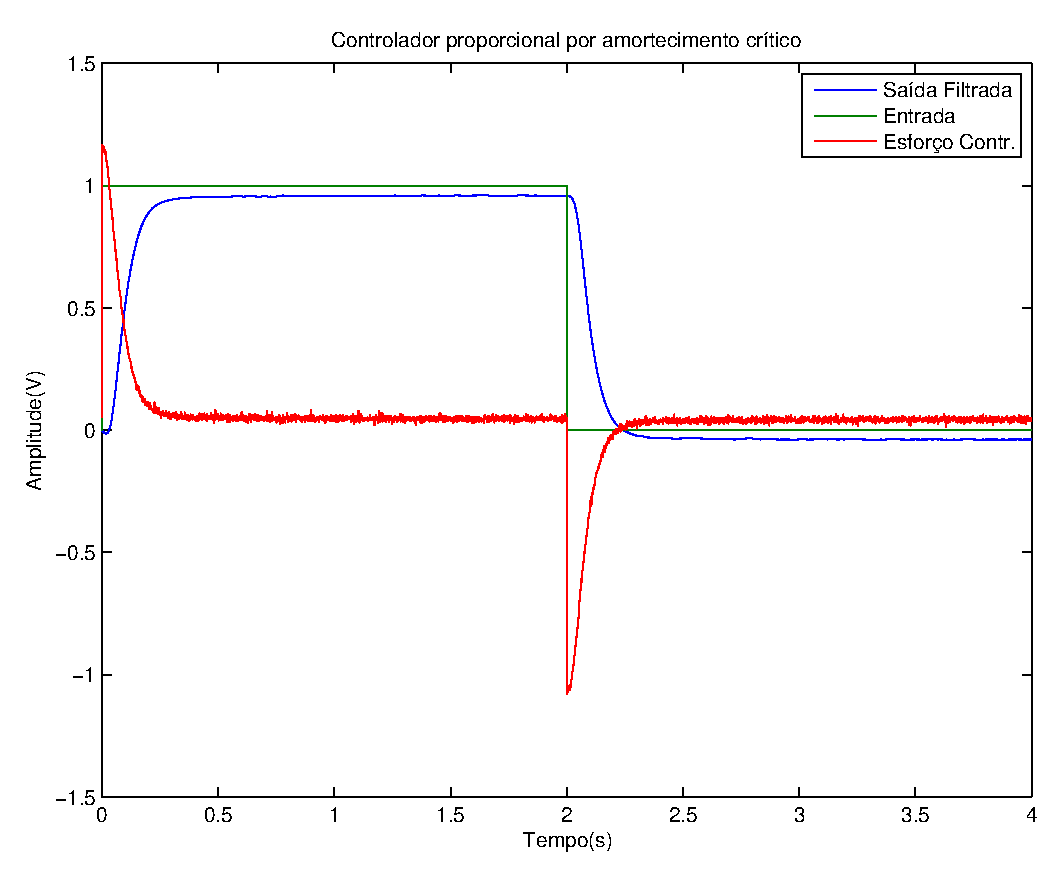
\includegraphics[width=0.8\linewidth]{yupidc}
 	\caption{Resposta filtrada e esforço de controle para onda quadrada do sistema com controlador projetado para amortecimento crítico}
 	\label{fig:ypidc}
 \end{figure}
Para esse controlador obtivemos as características apresentadas na tabela \ref{tab:pidc}
\begin{table}[H]
	\centering
	\caption{Características da resposta do sistema com controlador proporcional com amortecimento crítico}
	\label{tab:pidc}
	\begin{tabular}{|c|c|}
		\hline Característica & Valor \\ 
		\hline Tempo de estabilização & $0.2843$\\  
		\hline Sobrelevação & $0.3549\%$\\ 
		\hline Erro estacionário & $0.042$\\ 
		\hline 
	\end{tabular} 
\end{table}

Como podemos ver, a resposta desse controlador está bem próxima da resposta simulada representada na figura \ref{fig:simpidc}, porém o sistema apresenta um offset de $0.04 V$.
 \begin{figure}[H]
 	\centering
 	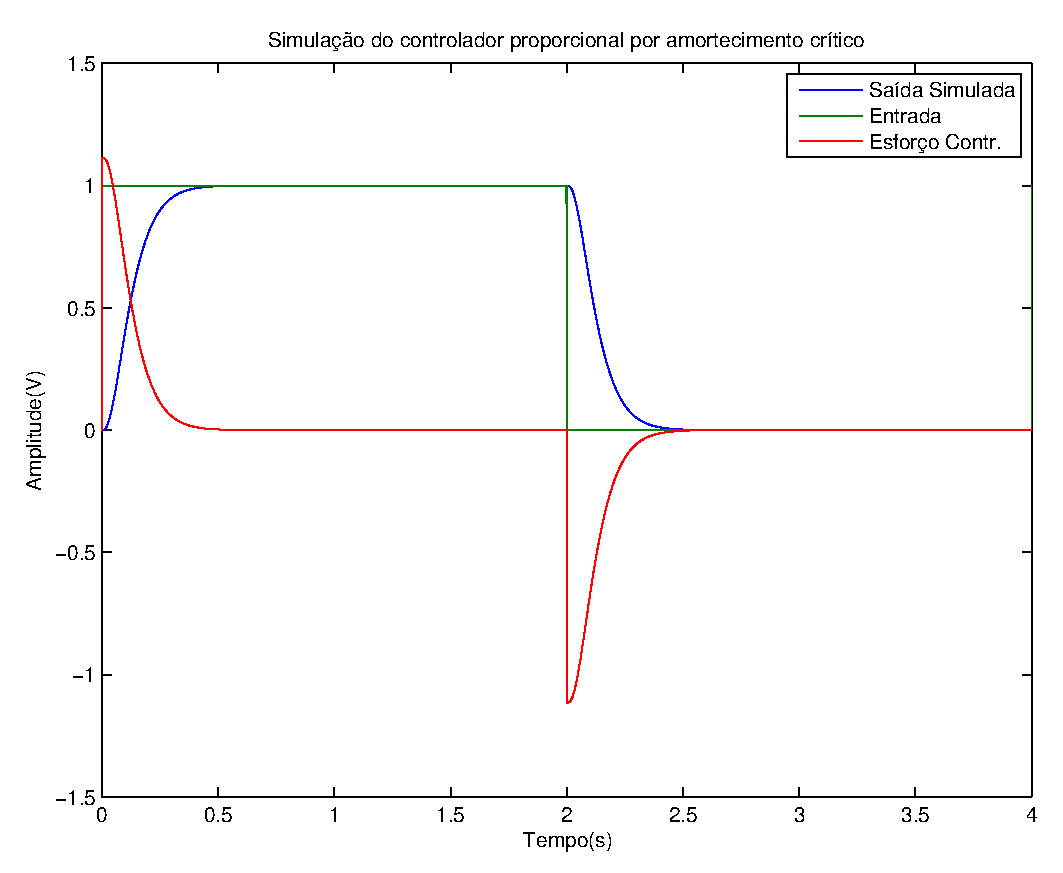
\includegraphics[width=0.8\linewidth]{yusimpidc}
 	\caption{Resposta e esforço de controle simulados para onda quadrada do sistema com controlador projetado para amortecimento crítico}
 	\label{fig:simpidc}
 \end{figure}
  
  \section{Controlador Proporcional com sobrelevação de 2$\%$}
  Outro controlador proporcional que foi projetado para obter o menor tempo de estabilização possível foi um controlador cuja sobrelevação é de exatamente $2\%$ de maneira à não sair do erro estabelecido. Esse controlador tem a seguinte função de transferência:
  \begin{equation}
  \label{eq:pidcv}
  C(s) = 1.609
  \end{equation}
  A resposta filtrada desse controlador à uma onda quadrada de amplitude $1 V$ e frequência de $0.25 Hz$ pode ser vista na figura \ref{fig:yupidv}.
  \begin{figure}[H]
  	\centering
  	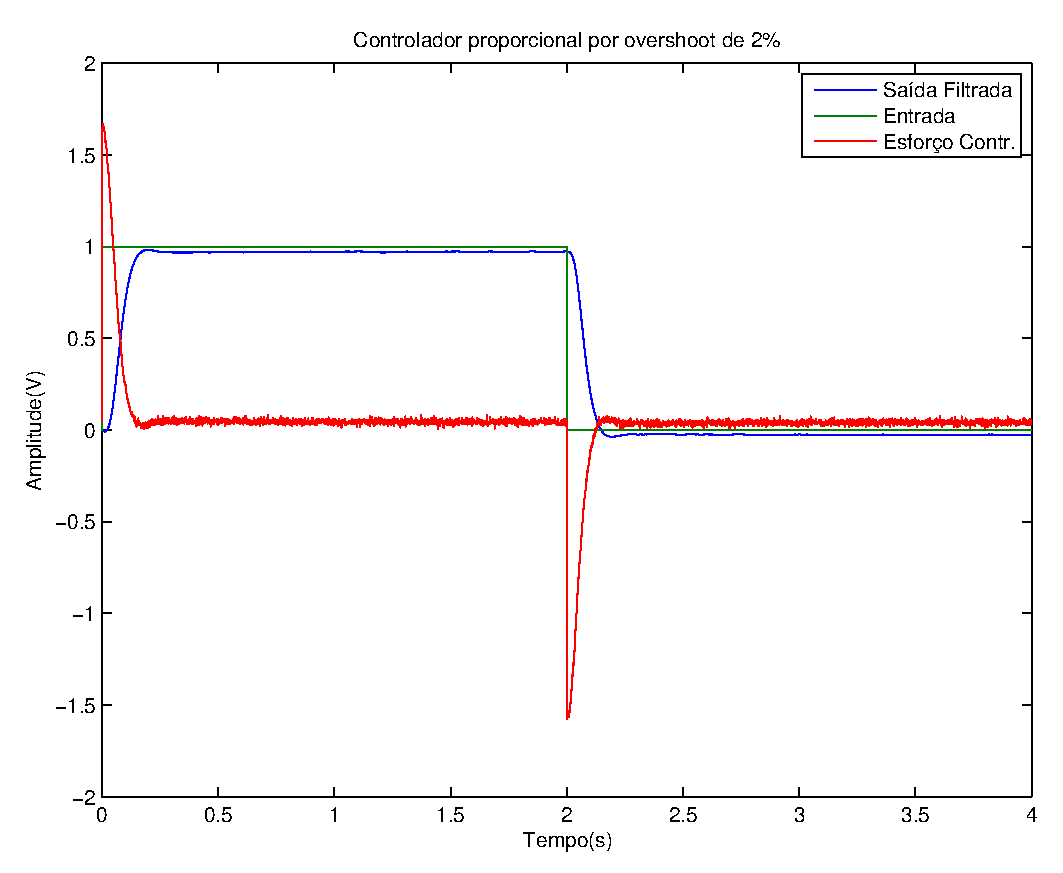
\includegraphics[width=0.8\linewidth]{yupidv}
  	\caption{Resposta filtrada e esforço de controle para onda quadrada do sistema com controlador projetado para sobrelevação de $2\%$}
  	\label{fig:yupidv}
  \end{figure}
  Para esse controlador obtivemos as características apresentadas na tabela \ref{tab:pidv} com o auxílio da função \textit{stepinfo} do Matlab.
  \begin{table}[H]
  	\centering
  	\caption{Características da resposta do sistema com controlador proporcional com sobrelevação de $2\%$}
  	\label{tab:pidv}
  	\begin{tabular}{|c|c|}
  		\hline Característica & Valor \\ 
  		\hline Tempo de estabilização & $0.1559$\\
  		\hline Sobrelevação & $0.96\%$\\ 
  		\hline Erro estacionário & $0.026$\\ 
  		\hline 
  	\end{tabular} 
  \end{table}
  
  Como podemos ver, a resposta desse controlador está bem próxima da resposta simulada representada na figura \ref{fig:simpidv}, porém o sistema apresenta um offset de $0.026 V$ e uma sobrelevação de somente $1\%$ diferente do projetado.
  \begin{figure}[H]
  	\centering
  	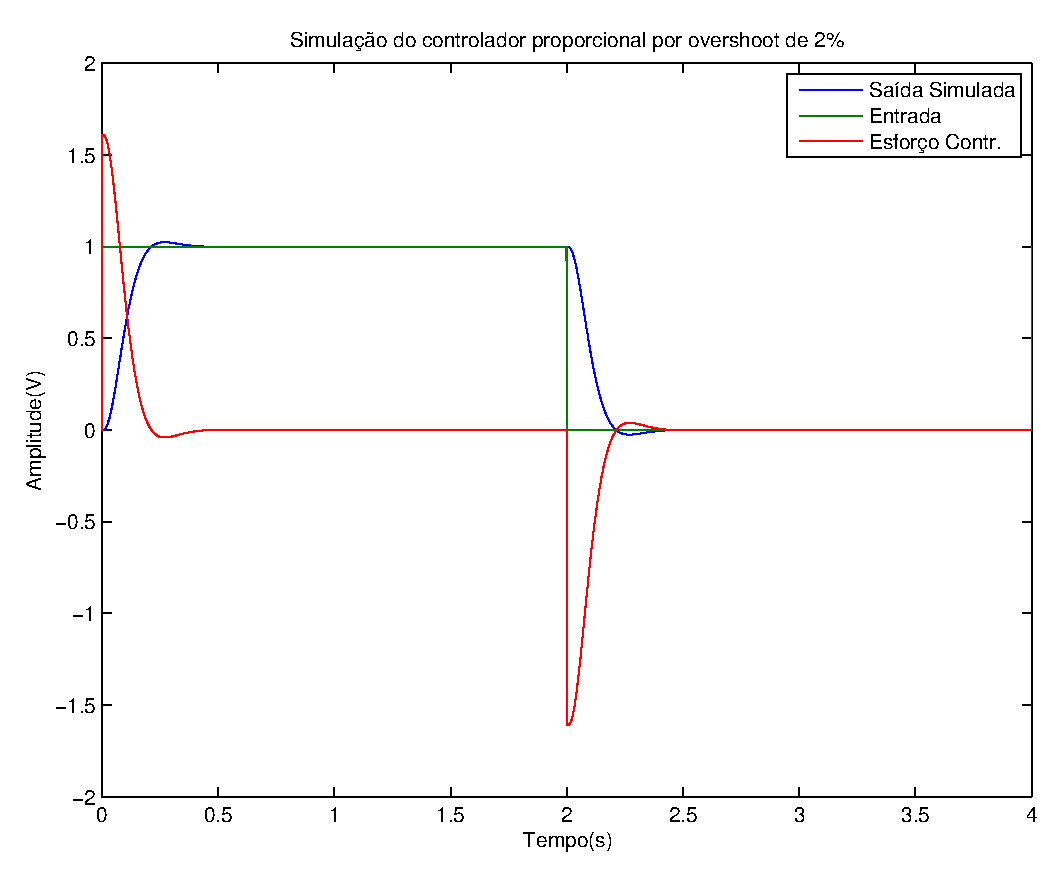
\includegraphics[width=0.8\linewidth]{yusimpidv}
  	\caption{Resposta e esforço de controle simulados para onda quadrada do sistema com controlador projetado para sobrelevação de $2\%$}
  	\label{fig:simpidv}
  \end{figure}
  
   \section{Controlador PID projetado pelo método Ziegler-Nichols}
   Esse controlador tem a seguinte função de transferência:
   \begin{equation}
   \label{eq:pidcz}
   C(s) = 9.05+\frac{142}{s}+0.144s
   \end{equation}
   A resposta filtrada desse controlador à uma onda quadrada de amplitude $1 V$ e frequência de $0.25 Hz$ pode ser vista na figura \ref{fig:ypidz} e seu esforço de controle na figura \ref{fig:upidz}.
   \begin{figure}[H]
   	\centering
   	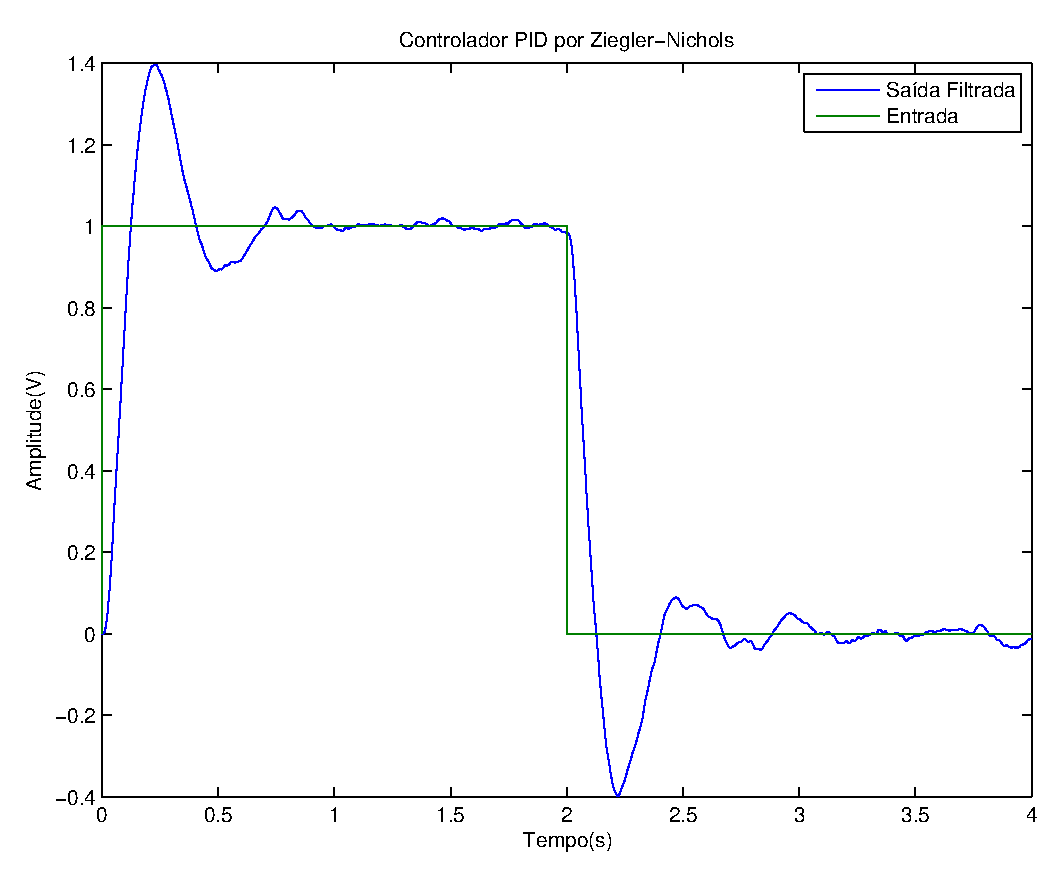
\includegraphics[width=0.8\linewidth]{ypidz}
   	\caption{Resposta filtrada à onda quadrada do sistema com controlador PID projetado pelo método Ziegler-Nichols}
   	\label{fig:ypidz}
   \end{figure}
   \begin{figure}[H]
   	\centering
   	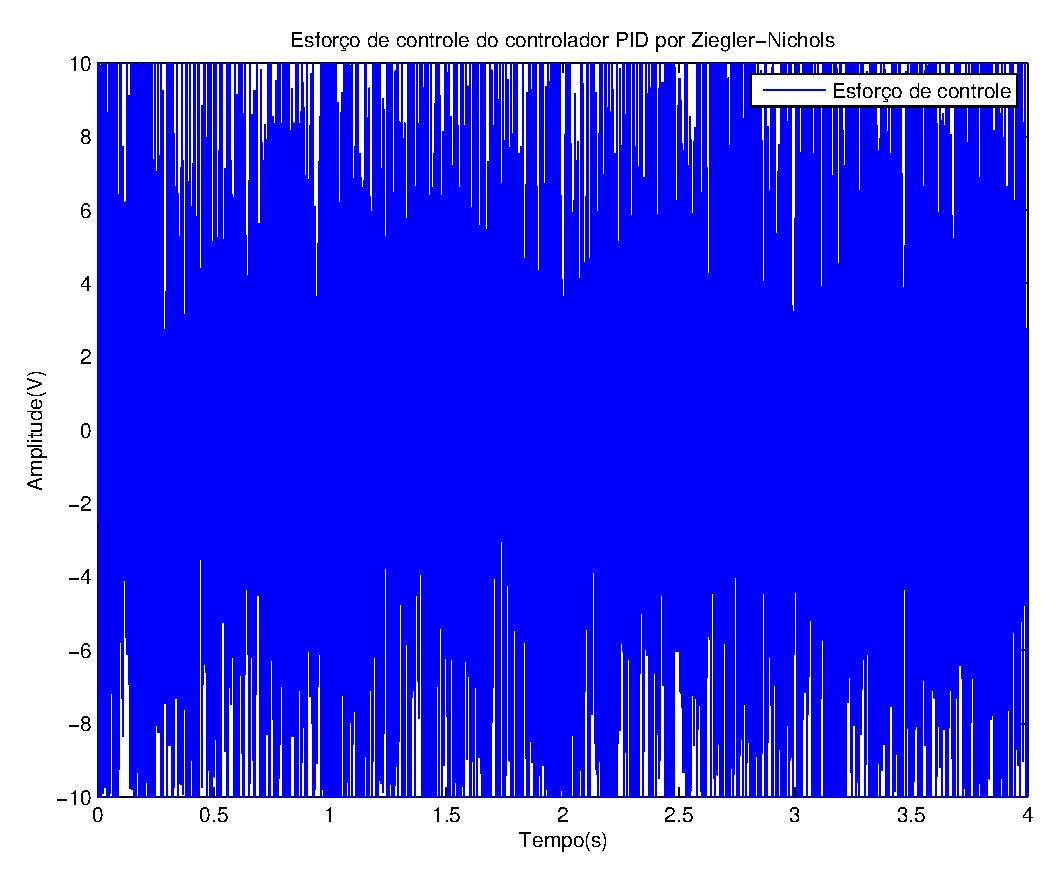
\includegraphics[width=0.8\linewidth]{upidz}
   	\caption{Esforço de controle para onda quadrada do sistema com controlador PID projetado pelo método Ziegler-Nichols}
   	\label{fig:upidz}
   \end{figure}
   Para esse controlador obtivemos as características apresentadas na tabela \ref{tab:pidz}
   \begin{table}[H]
   	\centering
   	\caption{Características da resposta do sistema com controlador PID projetado pelo método Ziegler-Nichols}
   	\label{tab:pidz}
   	\begin{tabular}{|c|c|}
   		\hline Característica & Valor \\ 
   		\hline Tempo de estabilização & $0.8789$\\ %TODO
   		\hline Sobrelevação & $39.69\%$\\ 
   		\hline Erro estacionário & $0$\\ 
   		\hline 
   	\end{tabular} 
   \end{table}
   
   Como podemos ver, a resposta desse controlador está próxima da resposta simulada representada na figura \ref{fig:simpidz}, porém seu esforço de controle é bastante diferente. Outra diferença esta no tempo de estabilização do sistema que é menor no sistema simulado. Acreditamos que as diferenças encontradas se devem principalmente à interferência de ruídos e as incoerências entre a função de transferência calculada para a planta e o sistema físico.
   \begin{figure}[H]
   	\centering
   	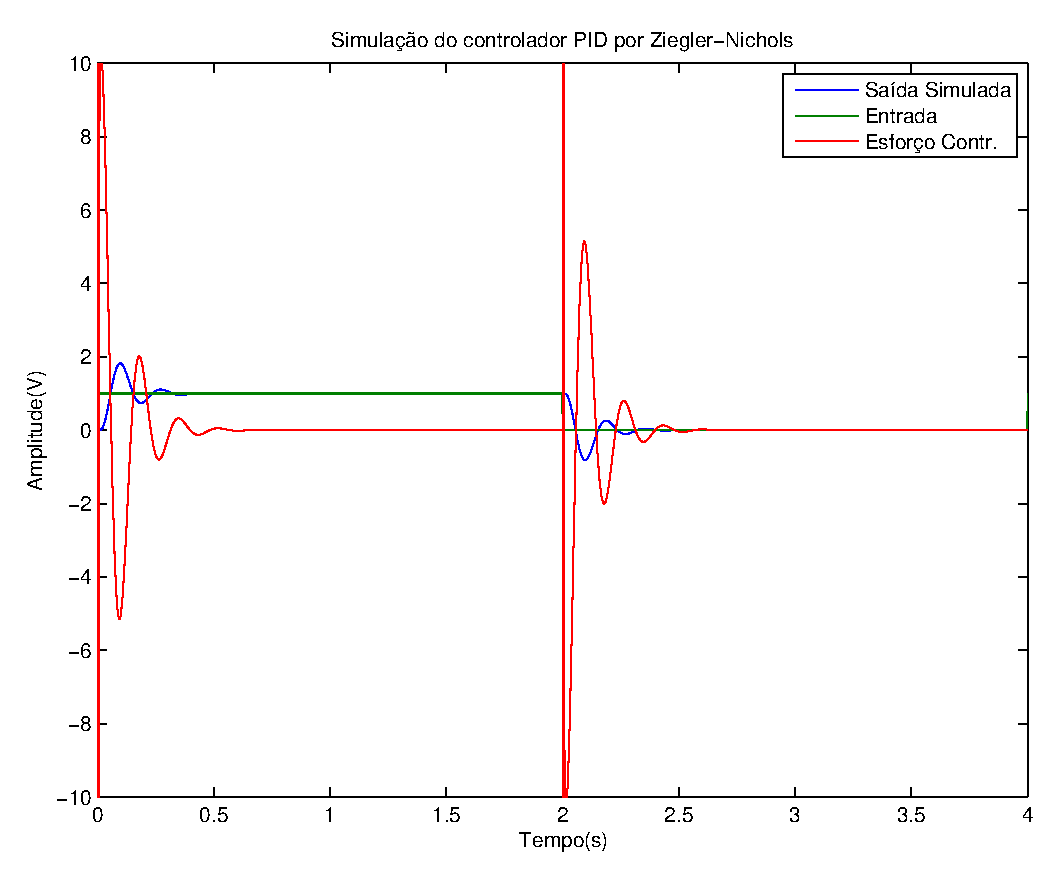
\includegraphics[width=0.8\linewidth]{yusimpidz}
   	\caption{Resposta e esforço de controle simulados para onda quadrada do sistema com controlador PID projetado pelo método Ziegler-Nichols}
   	\label{fig:simpidz}
   \end{figure}
   
   \section{Controlador PID projetado com o auxílio do SISO Tool}
   Utilizando a ferramenta SISO Tool, projetamos um controlador PID com a seguinte função de transferência:
   \begin{equation}
   \label{eq:pidcs}
   C(s) = 5.3+\frac{2.37}{s}+0.207s
   \end{equation}
   A resposta filtrada desse controlador à uma onda quadrada de amplitude $1 V$ e frequência de $0.25 Hz$ pode ser vista na figura \ref{fig:ypids} e seu esforço de controle na figura \ref{fig:upids}.
   \begin{figure}[H]
   	\centering
   	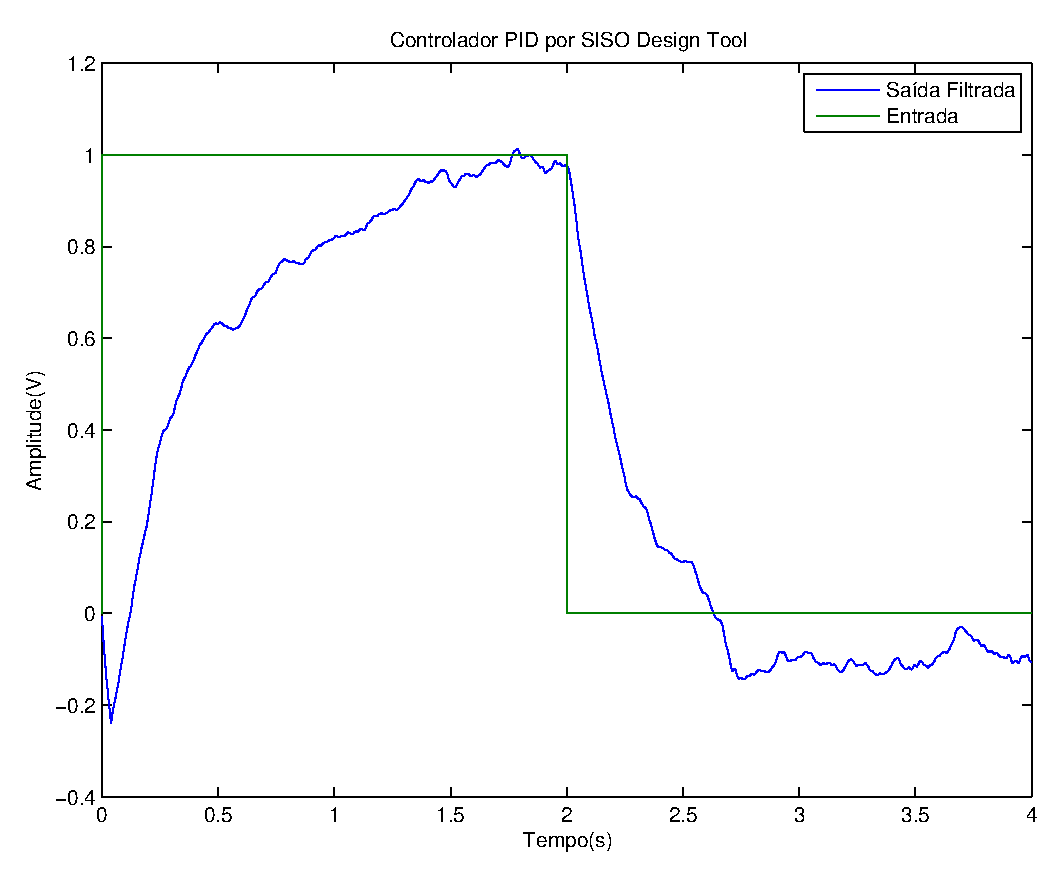
\includegraphics[width=0.8\linewidth]{ypids2}
   	\caption{Resposta filtrada à onda quadrada do sistema com controlador PID projetado com o auxílio do SISO Tool}
   	\label{fig:ypids}
   \end{figure}
   \begin{figure}[H]
   	\centering
   	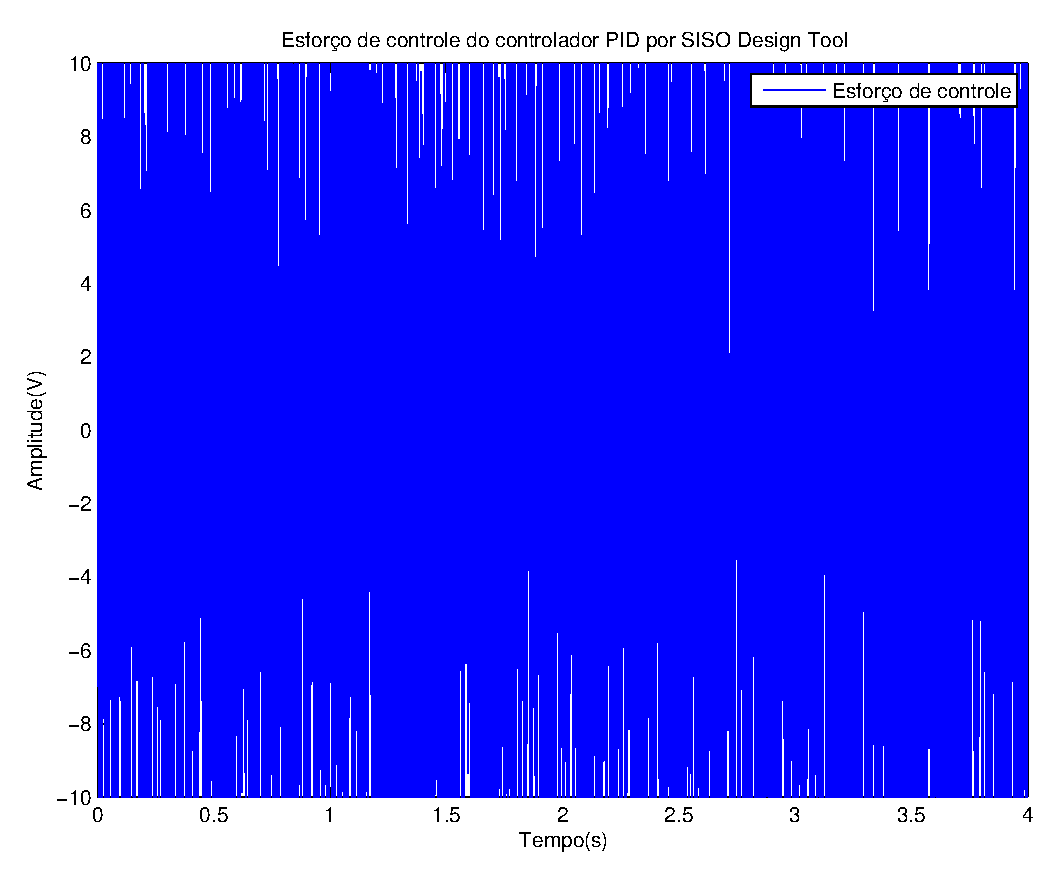
\includegraphics[width=0.8\linewidth]{upids2}
   	\caption{Esforço de controle para onda quadrada do sistema com controlador PID projetado com o auxílio do SISO Tool}
   	\label{fig:upids}
   \end{figure}
   Como podemos ver, esse controlador apresentou um desempenho insatisfatório e não é relevante analisar as características de sua resposta, como o tempo de estabilização ou erro estacionário. A resposta desse controlador está bem distante da resposta simulada apresentada na figura \ref{fig:simpids}. Acreditamos que essa diferença se deve à diversos fatores, notavelmente a falta de precisão na definição da função de transferência da planta e a interferência dos ruídos. Propomos como possível solução a filtragem do sinal de saída da planta antes de realimentar o controlador digital ou a utilização de um controlador analógico.
   \begin{figure}[H]
   	\centering
   	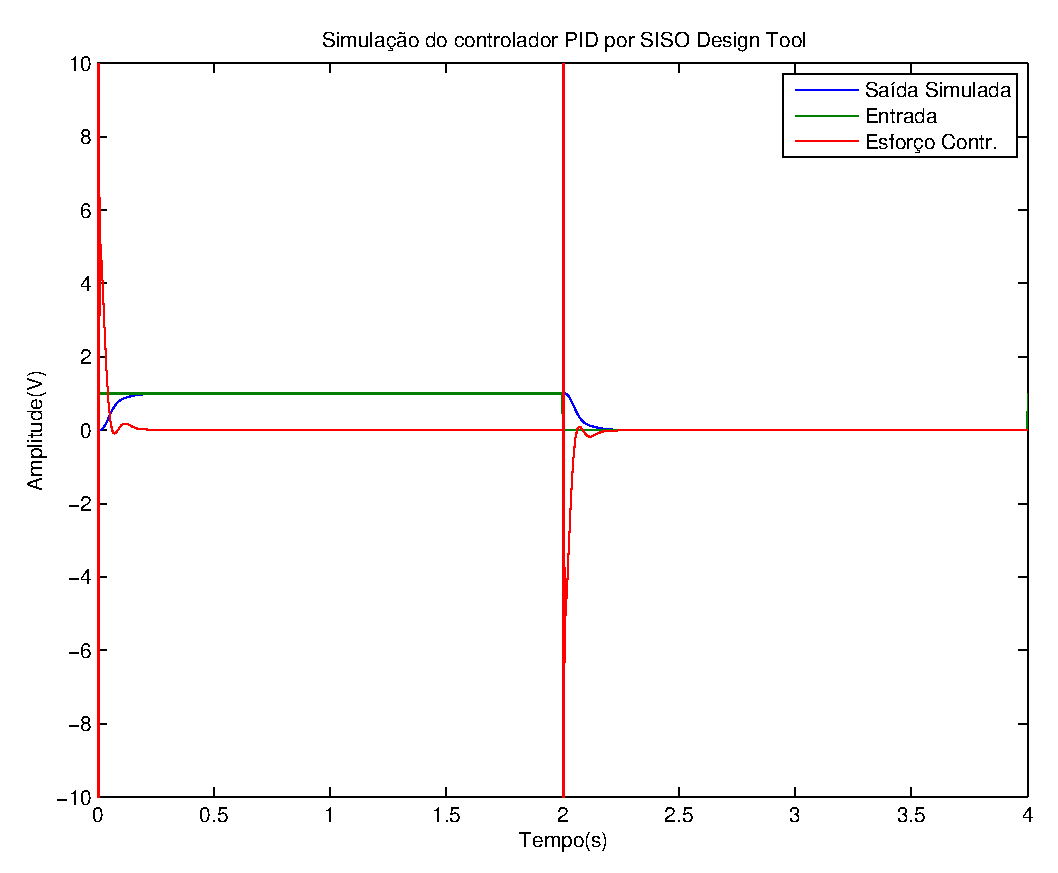
\includegraphics[width=0.8\linewidth]{yusimpids}
   	\caption{Resposta e esforço de controle simulados para onda quadrada do sistema com controlador PID projetado com o auxílio do SISO Tool}
   	\label{fig:simpids}
   \end{figure}
  
\begin{thebibliography}{widestlabel}
	\bibitem{bb:roteiro}{Roteiro do experimento disponibilizado para os alunos}
	\bibitem{bb:lab2}{KIAN, Marcelli; OLIVEIRA, Daniel. \textit{Relatório - Experimento 2:}Método de identificação de plantas eletrônicas}
	\bibitem{bb:prelab3}{KIAN, Marcelli; OLIVEIRA, Daniel. \textit{Pré Relatório - Experimento 3:} Controle de plantas eletrônicas utilizando um controlador PID digital.}
\end{thebibliography}
\end{document}

